% Synapse kan være sterkt basert på rapporter fra NEVR300[1,3,4] 

%KVIFOR I HELVETE skal han/vi gidde å lese om dette? Motiver leser of å lese om det biologiske systemet.
% Dette er også viktig for å "justify" neste kapittel - om modellering.
% 'Justification' skal hovedsaklig skje i forrige kap (ANN), og skal helst bare refereres til, her.







% TODO Skriv eksplisitt kvifor eg vil gå gjennom denne informasjonen så nøye.
% Eg skal prøve å holde implemensatjonene så lik biologien som mulig, for å beholde muligheten for å inføre nye konsept når desse blir funnet ut (av meg eller av neuroscience community).

%\chapter{Neuroscience: background information} %xxx rapport


\section{Biological Neural Systems} 
\label{secTheBiologicalNeuralSystem}
%Before we can discuss neural networks, either biological neural networks or artificial neural networks, we need to know more about the basic building blocks of the network. 
%TODO TODO TODO TODO TODO TODO TODO TODO TODO TODO TODO TODO TODO TODO TODO TODO TODO TODO TODO TODO TODO TODO TODO TODO TODO TODO TODO TODO TODO TODO TODO TODO TODO TODO TODO TODO TODO TODO TODO TODO TODO TODO TODO TODO 
% MÅ SKRIVES HEILT NY INNLEDING!
%TODO TODO TODO TODO TODO TODO TODO TODO TODO TODO TODO TODO TODO TODO TODO TODO TODO TODO TODO TODO TODO TODO TODO TODO TODO TODO TODO TODO TODO TODO TODO TODO TODO TODO TODO TODO TODO TODO TODO TODO TODO TODO TODO TODO 
In biology, neural networks are comprised of nodes called neurons and connections between the neurons, called synapses. 
Because the focus of this report is Artificial Neural Networks, only the aspects considered important to signal processing will be covered in this section.

When the neuron is to be used for pragmatic simulations, e.g. for filtering input or other technology related uses, a simple model has to be used.
In this simple model, only the most relevant aspects of the neuron is to be simulated.
We therefore use only one variable to define the state of the neuron; The membrane potential, also called ``the depolarization'' of the neuron.

The model most commonly used is the ``Leaky Integrate and Fire''(LIF) model\cite{florian03}. 
As the two compared designs are based on the LIF model, a special emphasis is put on the mechanisms important in this model; Synaptic integration and the leakiness of the value.
%As both the compared the designs are based on the LIF model, a special focus is put on the mechanisms of the neuron with respect to synaptic integration and the leak of the value of the neuron.
%With the value of the neuron it is referred to the ``depolarization'', or membrane potential of the neuron.

%The architecture of the neuron is impotant for understanding the different aspects of the neural network.
As we will see in this section, both the signalling in the synapse and the intracellular signal propagation of the neuron is directional;
	The signal comes in to the neuron at one end and exits at the other.
A network of neurons can therefore also be called a directional graph.
%This is one motivation for learning about the mechanisms of the neuron. %JEJEJE XXX XXX XXX Faen, trøtt.
%Whe can therefore define the graph as being directional.

The prime motivation for learning about the neuron is, however, that the design of the two models that are to be compared in this report is based on biology.
%An other motivation for introducing the biological neuron is that the design of both models is based on biology.
An understanding of the biological neuron will therefore make it easier to follow later sections.
When the design of each implementation is introduced, this section can also be used as a referere work.





%I will start by describing relevant information about the neuron before I prepare the reader for important aspects of synaptic plasticity by describing the synapse. Finally, important aspects of the network will be described.

%TODO Skriv om neuronet(overordna) i section: Biological Neural System} og skriv heller subsection{soma}
%TODO XXX XXX XXX SKRIV neuron inneholder soma,dendritt,axon,(synapser). subsubsection{kvar av desse}
\subsection{The neuron}
\label{ssecTheNeuron}
In mathematical terms from graph theory, a biologically realistic artificial neural network is a directed cyclic graph. 
In terms from neuroscience this meens that the network og neurons is recurrent (with feedback connections) and that the synapses (the connections between neurons) are directional --- information flows in one direction. 

%The majority of neurons in a biological being are so-called interneurons. This group of neurons have nervous input and give theire output to other neurons. 
%The biological neuron is special kind of cell with the ability to assess incoming inforamion and transmit information. 

%TODO fortsett på graph-sjargongen!
The neuron is surrounded by the cell membrane. This membrane has low permeability to ions from the fluid surrounding the neuron to the intracellular fluid of the neuron.
We also have ion pumps that pushes the ions ``upstream'' in relation to the electrical potential of the ionic concentration gradient.
%In addition we have different ionic pumps that pumps different ions from one side of the membrane to the other. 
This creates a difference in electrical charge, giving the electric potential over the membrane.
The membrane potential typically is around $-70mV$ at rest. %typically ligger feil (?).

%Maintaining this electrical potential is an energy demanding affair, and the brain uses about one fifth of the total $O_2$ use of the body. 

When the neuron gets an excitatory transmission through one of its input synapses, the neuron is said to become \emph{excited}. 
As an excitatory signal is one that makes the membrane potential more positive, this is also referred to as \emph{depolarizing} the neuron.
%This is also called being \emph{depolarized} as the potential goes to a less negative value. 
When the neuron gets a membrane potential that is more positive than the firing threshold, an action potential is initiated.
This is referred to as ``firing an action potential''.
The mechanisms behind the action potential is covered in sec. \ref{ssecTheActionPotential}.

\begin{figure}[hbt!p]
	\centering
	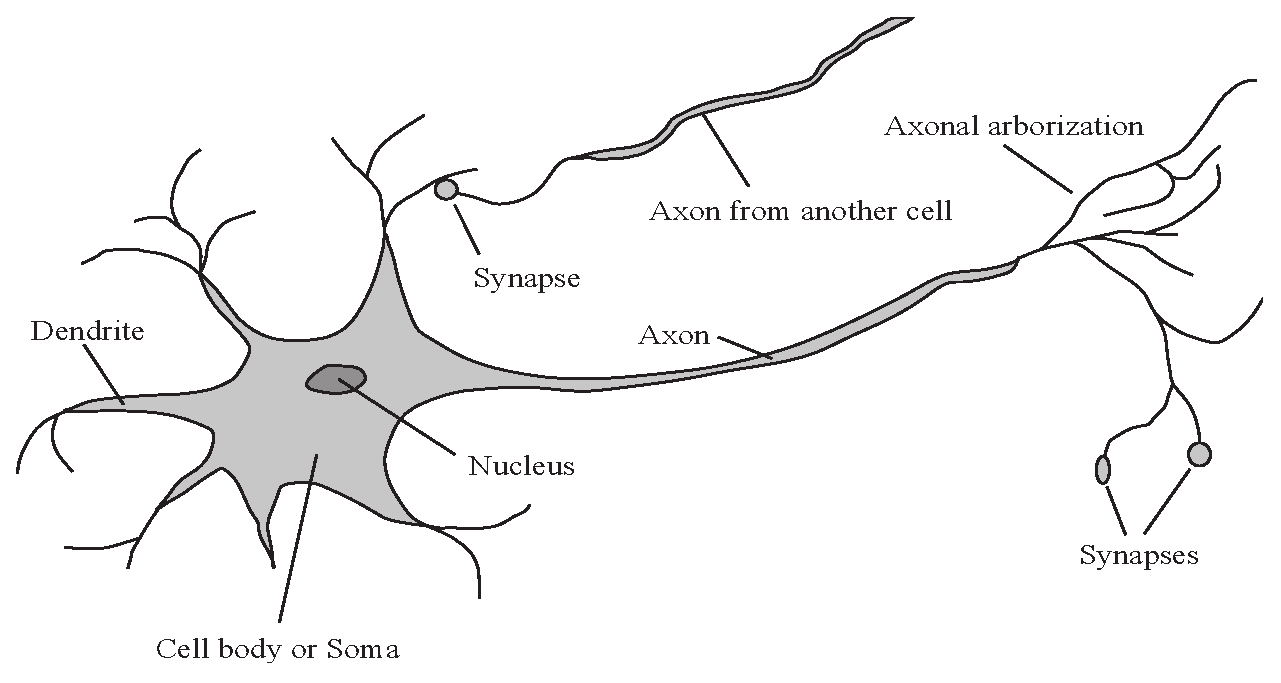
\includegraphics[width=0.95\textwidth]{ModellAvNeuronet.eps}
	\caption{A illustrative model of the neuron. The signal propagation goes from the left to the right in this figure;
			Synaptic integration at the dendrites, action potential through the axon and finally transmission throught the output synapses. 
			The aspects of the cell body is not immediately relevant to signal processing, and is not taken into account in the model used. }
	\label{figFigurAvNeuronet}
\end{figure}

% Gjennomgang, natt til 30juli. Her er eg no.
% TODO TODO TODO TODO TODO TODO TODO TODO TODO TODO TODO TODO TODO TODO TODO TODO TODO TODO TODO TODO TODO TODO TODO TODO TODO TODO TODO TODO TODO TODO TODO TODO TODO 

When the action potential reaches the ``axon terminal'', where the presynaptic membrane of the synapse lies, neurotransmitters are released into the synaptic cleft 
 	(se appendix \ref{appendixSecPresynapticSynapticPartOfTransmission} for a more complete discussion of the action potential and the presynaptic elements of synaptic transmission).
The neurotransmitters diffuse passively out in the synaptic cleft. Some come in contact with the postsynaptic receptors, and activates the receptor.
%The receptors that are relevant to this project is the ligand--gated receptor group.
%Describing the different known kinds of receptors will be outside the scope of this report. We will limit the description to one class of receptors, called ``ligand--gated receptors''.
Directly--gated receptors (also called ``ligand--gated channels'') open a channel when exposed to the right ligand (the right neurotransmittor), 
	causing an increase or decrease in the postsynaptic neurons depolarization\cite{PrinciplesOfNeuralScience4edKAP10}. .
%Ligand--gated receptors are direcly connected to ion channels in the membrane. Opening of these ion specific channels enables some ions to flow throught (depending on what kind of channel the receptor is connected to). 
%Depending on which ions are let through, the neuron is either depolarized (towards zero polarization, less than its resting potential) of hyberpolarized (getting a more negative membrane potential) by the transmission.
Whether the postsynaptic depolarization is increased or decreased by a synaptic transmission defines the synapse as being an excitatory or an inhibitory synapse\cite{PurvesNeuroscienceKAP05}.
%On the postsynapsic membrane in the synapse are different receptors for different neurotransmitters\cite{PrinciplesOfNeuralScience4edKAP10}. 
%The receptors are only activated by some neurotransmitters, and the change in postsynaptic postential varies with what ions the receptor channel is permeable to.

%Since depolarizing the neuron causes firing, the neurons potential is often referred to as the neurons depolarization in the litterature.



\subsection{The Axon and the Action Potential}
\label{ssecTheActionPotential}
In the membrane of the axon we have voltage--gated channels that open if the level of depolarization is more than some value. This value is called the ``firing threshold of the neuron''.
These channels will open and further depolarize the membrane. 
Through passive transmission of the electrical potential, the next voltage gated channels will open as a result of going above the gate threshold. %also go beyond the firing threshold.
This establishes the active aspect of action potential propagation, and results in a self carrying propagating through the axon.
%This establishes the self carrying signal of the axon, and results in an equal depolarization at the different axon terminals\cite{PrinciplesOfNeuralScience4edKAP09}.
An important result of this is that the presynaptic membrane at the synapses recieves an equal depolarization, independent of its location. 
The release of neurotransmitters is a result of this depolarization, and the action potential enshures an equal depolarization of the presynaptic membrane.
This gives that the transmission is dependent only on the synaptic connection, or ``the synaptic weight''\cite{PrinciplesOfNeuralScience4edKAP09}.
%
%This means that sufficient depolarization of the membrane of the axon opens voltage gated ion channels that will further depolarize the membrane. 
%Through passive transmission of the voltage, the signal is distributed to the next voltage gated channels.

%todo skriv mot slutten av paragraf:  The voltage gated channels will only be open for a small period of time.
%There are at multiple kinds of voltage gated channels. The sodium channel opens
For the action potential there are two important voltage--gated channels; The sodium channel and the potassium channel.
The $Na^{1+}$ channel opens faster than the $K^+$, and gives the rising phase of the action potential.
The rising phase of the action potential comes as a consequence of more positively charged $Na^{2+}$ ions outside the neuron causing a strong inward current after opening of the $Na^{2+}$ channels.
Voltage gated $Na^{2+}$ only stay open for about 1 ms before they close.
About the same time as the $Na^{2+}$ channels close, the $K^+$ channels open. 
Because there is a larger concentration of $K^+$ inside the cell, this will cause a more negative potential over the membrane. The neuron is repolarized.
%After some time delay, the $K^+$ channel opens, and at about the same time the $Na^{2+}$--channel close.
%We have more $K^+$ ions inside the cell, so increasing the permeability for $K^+$ will decrease the depolarization over the membrane, or ``repolarize'' the membrane.
%When both channels are closed again we are back at the resting potential of the neuron. %SITER: Bear s:91
After the action potential the membrane potential is ``reset''.
As the electrical potential spead passively to the next site with voltage--gated channels, 
	the refraction period of each voltage gated channel is an impotant mechanism to hinder the action potential from going ``the wrong way''\cite{NeuroscienceExploringTheBrain3edKAP4}\cite{PrinciplesOfNeuralScience4edKAP09}.

To recreate the ionic gradient, the ions are transported back by the sodium--potassiom pump.
As this is a mechanism that use a little time to reset the ionic gradients, we have a little period when the gates have to be closed.
This is the basis for the refraction period of the neuron, a small period of time where action potential cannot be initiated\cite{NeuroscienceExploringTheBrain3edKAP4}.

After firing an action potential, the neuron will also have a short period where it is impossible to exite the cell, called \emph{the absolute refraction period}\cite{PrinciplesOfNeuralScience4edKAP09}.. 
%The refraction period of a neuron usually lasts for a few milliseconds\cite{PrinciplesOfNeuralScience4edKAP09}.
%\cite Bear kap. 4  (s.91, nede) og Kandel kap.9 s 157 (nede)
%TODO TODO TODO TODO TODO TODO TODO TODO TODO TODO TODO TODO TODO TODO TODO TODO TODO TODO TODO TODO TODO TODO TODO TODO TODO TODO TODO TODO TODO TODO TODO TODO TODO TODO TODO TODO TODO TODO TODO TODO TODO TODO TODO TODO 
% Plan: finn referanse på dette, og så sei at eg har matematisk vist det å være sant.
In this project, the author has demonstated matematically that the refraction period is important for limiting the firing frequency of the neuron. 
The analysis is presented in section \ref{ssecValueOfAlpha}.
%In this project the author has formalized that the refraction period is important for limiting the firing frequency of the neuron. The analysis is presented in section \ref{ssecValueOfAlpha}.


%												"close to":  SKRIV OM
The axon is organized as a tree, with a trunk in close proximity to the soma of the neuron, called the axon hillock.
The branches of the ``axonic tree'' are called axon collaterals. 
The elements of the axon that is furthest from the axon hillock is called the axon terminal, and is where the output synapses are located.
%The axon ``ends'' in the axon terminal, where the presynaptic part of the synapse is located.
When the action potential reaches the synapse, a transmission is initialized by the opening of voltage gated $Ca^{2+}$ channels\cite{PrinciplesOfNeuralScience4edKAP10}.
%The signals transmitted in the axon is strictly directional, that is: the signal goes from the axon hillock (close to the neurons soma) to the axon terminals (where the synapses is). 

%ODO Skriv mindre, eller i det minstre mindre kraftige utsagn. Følgande er rett, men kanskje urelevant for denne oppgava?
%You also have modulatory synapses at the axon terminal, that does not contribute to the value of the neuron, only the amount of neurotransmitters released following the next incoming action potential. 
%The modulatory synapse is but an example of the complexity of the simplifications that are neccesary in order to make an artificial neural network.
%In addition we have different time delay for different synapses along the axon, diffuse modulatory systems it the brain with modulatory neurotransmittors, 
%different states as the neurons use the oxigene and nutritients available, etc.






\subsection{The synapse}
\label{ssecTheSynapse}
%\subsubsection{Synaptic Plasticity}
%When the action potential reaches the axon terminal, the size of the signal is thought to be the same as when it first was initialized at the axon hillock.
%This enshures that the distance the action potential has to travel does not affect the transmission at the synapses of the different axon terminals. \cite{NeuroscienceExploringTheBrain3edKAP4}.
Following an action potential, voltage gated $Ca^{2+}$ channels are opened and $Ca^{2+}$ enters the axon terminal.
This causes synaptic vesicles to merge with the presynaptic membrane, causing the content of the synaptic vesicles to be released into the synaptic cleft. %Cite Kandel kap.10
% Forrige to linjer (passer med siste forrige section) ELLER neste linje:
%When an action potential reaches the location of a particular synapse, the membrane potential will cause release of neurotransmittors from the axon terminal (the presynaptic neuron).
%-------------------------------------------------------------------------ordna til hit-------------------------------------------------------------------------------------------------------------------------------------------
The neurotransmitters from the synaptic vesicles diffuse into the synaptic cleft.
If a so--called ligand--gated channel at the postsynaptic membrane is exposed to these neurotransmitters, the channel opens and ions are let thought.
The result is either excitation or inhibition of the postsynaptic node's value, depending on the channel (which ions are let through).
The size of the transmission is based on presynaptic and postsynaptic mechanisms\cite{PurvesNeuroscienceKAP05}.
%The transmission is thought to be a funcion of presynaptic and postsynaptic mechanisms.

\begin{itemize}
	\item Presynaptically, different amount of neurotransmitters can be released from the axon terminal following an action potential.
	\item Postsynaptically, the amount of receptors varies between different synapses. The amount also varies with time. % This is one mechanism of synaptic plasticity.
\end{itemize}

The level of transmission is the background for what is modelled as the synaptic weight in artificial neural networks.
%These two sides of synaptic transmission are important when synaptic plasticity is considered. 
Patterns of long term synaptic plasticity is what is what is percieved as learning in the field of neuroscience \cite{NeuroscienceExploringTheBrain3edKAP25}.
A more comprehensive study of synaptic plasticity is outside the scope of this text, but it should be mentioned that the ion $Ca^{2+}$ is thought important in both presynaptic and postsynaptic plasticity.
The postsynaptic role of $Ca^{2+}$ is important for STDP, which is an important argument for ANN with the capability of calculating the spike time.
%This is important for STDP, which is an important argument for ANN with the capability to calculate the timing of the spike.
For the especially interested, appendix \ref{appendixSynPlast} considers presynaptic and postsynaptic mechanisms behind synaptic transmission and synaptic platicity, with a special focus on the role of $Ca^{2+}$.








% //{ Kommentert ut.  Gave til meg selv når eg skal skrive masteren (liten gave, nesten ingenting)

% //{
%The conclution from the study about 

% % XX MED-noke-om: For now, it is enough to mention that the synaptic weight changes as a multifactorial function based on 
%For now, it is enough to mention that  $Ca^{2+}$ is important both presynaptically and postsynaptically for synaptic plasticity.
% % We will later make use of some of the 
% % XXX Bra, men passer det inn:
%When the action potential reaches the axon terminal, it will open voltage--gated $Ca^{2+}$ channels in the active zone of the terminal, and $Ca^{2+}$ enters the cytosol of the axon terminal of the presynaptic neuron\cite{PrinciplesOfNeuralScience4edKAP10}.












% The signal arriving at the presynaptic membrane is equal for all the synapses, the transmission is not. 
% The transmission varies as a function of many mechanisms. %xxx Dårlig setning!
% For the scope of this text, we will focus on the mechanisms within the neuron. 
% I will refer to the size of this transmission as the weight of the synapse. 
% % Dårlig skrevet, over her.

%In this report the convention used by Rolls and Treves in ``Neural Networks and Brain Functions'' will be used. 
%For any transmission through a synapse between neuron $j$ and neuron $i$, we define the synaptic strength $w_{ij}$. 
%Note that the first subscript refers to the recieving neuron and the last subscript to the presynaptic neuron (the signalling neuron) \cite{TrevesNeuralNetworks}.
%This convention will be used in this text. 







%This does not mean that the transmission for different synapses is the same. At each synapse the connection to the postsynaptic neuron is different. 
%There are many mechanisms behind this, but I will focus on the mechanisms within the neuron:
% //}

%\subsubsection{Presynaptic mechanisms behind synaptic plasticity}
% //{
%$Ca^{2+}$ causes release of neurotransmittors from the presynaptic axon terminal into the synaptic cleft\cite{PrinciplesOfNeuralScience4edKAP10}. 
%Long--term potentiation (LTP) causes a lasting change of the tranmission through the synapse.% On the shorter time scale we have short--time potentiation, called fascilitation and short--time depression (decrease of transmission) called 
%
%The amount of $Ca^{2+}$ inflow, and thus the amount of neurotransmitter release can be modulated by socalled axoaxonic synapses\cite{NeuroscienceExploringTheBrain3edKAP5}, synapses that is connected directly to the presynaptic axon terminal. 
%A transmission here will cause a small increase in the axon terminals amount of $Ca^{2+}$ and ``prime'' the synapse for a transmission. 
%Multiple incoming action potentials in fast succession will have the same effect on the following action potentials and causes what is called \emph{potentiation} (short term increase in synaptic weight)
%\cite{PrinciplesOfNeuralScience4edKAP14}. 
% %Variation of the $Ca^{2+}$ entering the presynaptic axon terminal, for example by ``priming'' the synapse for transmission by axon-synaptic synapses, is one potential mechanism for synaptic plasticity\cite{PrinciplesOfNeuralScience4edKAP14}.

% X XX Ta vekk mykje av "Presynaptic mechanisms behind synaptic plasticity" om eg ikkje bruker desse effektene i implementasjonen!
% //}


%\subsubsection{Postsynaptic mechanisms behind synaptic plasticity}
% //{
%Glutamate is the main excitatory neurotransmittor in the CNS\cite{PrinciplesOfAnatomyAndPhysiology12edKAP12}. %s. 448
%There are two main groups of ligand--gated glutamate receptors, the N-methyl D-aspartate (NMDA) receptors and the non-NMDA receptors. 
%The non-NMDA receptors mainly consists of the $\alpha$-amino-3-hydroxy-5-methyl-4-isoxazolepropionic acid (AMPA) receptor. %XXX SITER!
%
%Most non-NMDA receptors are permeable to ions that changes the postsynaptic potensial without having lasting changes on the synaptic strength.%efficiancy. 
%The NMDA receptor is permeable to $Ca^{2+}$, which is important for lasting changes of the synaptic strength. %uttrykket 'synaptic strength' har ikkje blitt definert enda. Gjør det lenger oppe. XXX DO IT!
%
%An other important difference between the NMDA-R and the AMPA-R is that NMDA receptors have an additional condition for opening of its ion channel. 
%In the NMDA receptor there is a $Mg^{2+}$ ion blocking the channel. 
%When the potential across the membrane is sufficiently depolarized, the $Mg^{2+}$ will float more freely and the block is removed from the NMDA receptor.
%$Ca^{2+}$ diffuses into the cell following an action potential\cite{PrinciplesOfNeuralScience4edKAP12}.
%
%Also on the postsynaptic part of the synapse $ca^{2+}$ has an important role in synaptic plasticity. 
%$Ca^{2+}$ activates production of more non-NMDA receptors for the postsynaptic membrane, resulting in LTP\cite{AMPARtrafficingArtikkel}.%\cite{PrinciplesOfNeuralScience4edKAP12}.
%
% %TODO Det under gjelder jo bare for kvifor vi får positiv vektendring. Skriv dette, eller finn ut forklaringa for negativ vektendring (LTD) som følge at STDP! XXX
%The NMDA-related synaptic plasticity is the background for what is called ``Spike Timing Dependent Plasticity'' (STDP) that will be important later in this text.
% % XXX ikkje "rest of this text." Det er ikkje viktig over alt. Noken plasser.. Kanskje "an important element in this text."?
% %Skriv om hebbian learning, ustabilitet  og at STDP kalles "stable hebbian learning". Sjå rapport i NEVR3004.
% %STDP has also been called ``stable hebbian learning''. This refers to the 

%\subsection{SKRIV OM STDP! Referer til forrige avsnitt}
% %TODO: sjå rapport NEVR3001, NEVR3003.
% %HER ELLER OVER. kjør \label{forklaringBakSTDP}
% //}

%\label{forklaringBakSTDP} %der forklaringa kommer...

%\subsection{Skriv om Dale's  principle}
%At eit neuron kan sleppe bare en neurotransmittor (eller to, fleire). Desse kan gi ulik virkning på ulike receptore, men i utgangspkt. kan man sei at eit neuron enten er excitatory eller inhibitory. 
%Men dette er også feil. Drøft fram og tilbake.. Skriv konklusjonen (til korleis eg gjør det i min implementasjon) i section{implementation}.


% %Because of the boolean nature of the action potential, the transmission of the action potential to the next neuron is desided by the strength of the synaptic connection.

% %The most studied neurotransmittor is glutamate. In most neurons glutamate is an excitatory 

% %Skriv om STDP (glutamate), om bakgrunnen for STDP: NMDA med mg²⁺ blokk, voltage dependent i tillegg til at utsida må være eksponert for glutamat, Ca²⁺ inflow fører til AMPA-syntese => synaptisk plastisitet! 


%\subsection{nettverket}
% - Med booleanske signal: korleis kan signalet inneholde så mykje informasjon?
% 		- skriv om inter-spike period. Og kanskje om ANN-flyttals variablene som output fra neurona..
% //}
